\documentclass{beamer}

% Copyright 2010 Drow Ltd.
% 
% In principle, this file can be redistributed and/or modified under
% the terms of the GNU Public License, version 2.
% 
% However, this file is supposed to be a template to be modified
% for your own needs. For this reason, if you use this file as a
% template and not specifically distribute it as part of a another
% package/program, I grant the extra permission to freely copy and
% modify this file as you see fit and even to delete this copyright
% notice. 
\mode<presentation>
{
  \usetheme[titleline=true,
  alternativetitlepage=true,
  titlepagelogo=images/Java_logo]{Torino}
  \usecolortheme{nouvelle}
  \beamertemplatenavigationsymbolsempty
}

\usepackage{times}
\usepackage[utf8]{inputenc}
\usepackage[english,bulgarian]{babel}
\usepackage[T2A]{fontenc}

\usepackage{listings}
\lstset{language=Java,
  captionpos=b,
  tabsize=4,
  keywordstyle=\color{blue},
  commentstyle=\color{gray},
  stringstyle=\color{green},
  numbers=left,
  breaklines=true,
  showstringspaces=false,
  basicstyle=\ttfamily,
  emph={label},
  frame=shadowbox, 
  rulesepcolor=\color{blue},
  columns=fixed}

\title{Увод в създаването на графични потребителски интерфейси със Swing}

\author{инж. Божидар ~Бацов}

\institute{Drow Ltd.}

\date{30.11.2010}

\subject{Talks}
% This is only inserted into the PDF information catalog. Can be left
% out. 

\begin{document}

\begin{frame}
  \titlepage
\end{frame}

\begin{frame}{Съдържание}
  \transdissolve
  \tableofcontents[pausesections]
\end{frame}

\section{История на GUI в Java}

\subsection{AWT}

\begin{frame}{В началото бе AWT}
  \transdissolve
  \begin{itemize}
  \item AWT - Abstract Widget Toolkit
  \item Част от Java 1.0
  \item Използват се компоненти от операционната система
  \item Ограничени възможности
  \item Неконсистентен краен продукт
  \item Write once, run everywhere се превръща в Write once, debug everywhere...
  \end{itemize}
\end{frame}

\subsection{Swing}
\begin{frame}{Swing}
  \transdissolve
  \begin{itemize}
  \item Netscape създава IFC(Internet foundation classes) през 1996
    \begin{itemize}
      \item компонентите изглеждат еднакво на всички ОС
      \item компонентите се рисуват от IFC
    \end{itemize}
  \item Swing - резултат от сътрудничество между Sun и Netscape
    \begin{itemize}
      \item разширение за Java 1.1
      \item част от Java 1.2
    \end{itemize}

  \end{itemize}
\end{frame}

\begin{frame}{Предимства на Swing}
  \transdissolve
  \begin{itemize}
  \item Голям набор от качествените стандартни компоненти
  \item Почти никаква зависимост към операционна система
  \item Консистентен краен продукт на различните платформи
  \item Контрол на външния вид на приложенията чрез Pluggable look and
    feel
    \begin{itemize}
      \item Metal(Java look and feel)
      \item Ocean(Java 1.5)
      \item Nimbus(Java 1.6)
      \item Third-party look and feels
    \end{itemize}
  \item Модел-изглед-контролер(Model View Controller) архитектура
  \end{itemize}
\end{frame}

\subsection{SWT}
\begin{frame}{SWT}
  \transdissolve
  \begin{itemize}
  \item SWT - Standard Widget Toolkit
  \item Разработен от IBM за проекта Eclipse
  \item Използва native(heavyweight) компоненти
  \end{itemize}
\end{frame}

\begin{frame}{Графичен потребителски интерфейс}
  \transdissolve
  \begin{itemize}
  \item Прозорец
  \item Декорация на прозореца
  \item Контроли
  \item Управление на разположението на контролите
  \item Реакция на потребителски вход
  \end{itemize}
\end{frame}

\begin{frame}{Структура на прозорец}
  \transdissolve
  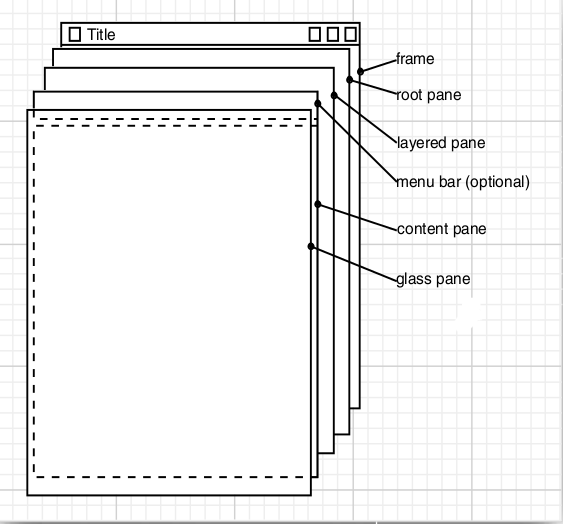
\includegraphics[width=320px,height=160px]{images/jframe.png}  
\end{frame}

\section{Компонентна йерархия}
\subsection{Frame}
\begin{frame}{Frame}
  \transdissolve
  \begin{itemize}
  \item Прозорец, който не се съдържа в друг прозорец
  \item Рисува се от ОС
  \item Frame != JFrame
    \begin{itemize}
      \item Frame - AWT
      \item JFrame - Swing
    \end{itemize}
    \item При създаването си НЕ Е видим!
  \end{itemize}
\end{frame}

\begin{frame}[fragile]
  \frametitle{Пример}
  \transdissolve
\begin{lstlisting}
public static void main(String[] args) {
   EventQueue.invokeLater(new Runnable() {
     public void run() {  
       JFrame frame = new JFrame();
       frame.setSize(600, 400);
       frame.setDefaultCloseOperation(JFrame.EXIT_ON_CLOSE);
       frame.setVisible(true);
     }
  });
}
\end{lstlisting}
\end{frame}

\subsection{Връзка между AWT и Swing}
\begin{frame}{Връзка между AWT и Swing - графика}
  \transdissolve
  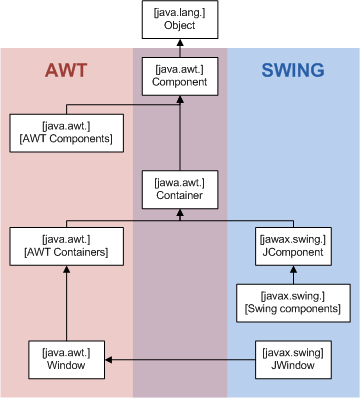
\includegraphics[width=320px,height=160px]{images/AWTSwingClassHierarchy.png}  
\end{frame}

\begin{frame}{Йерархия - графика}
  \transdissolve
  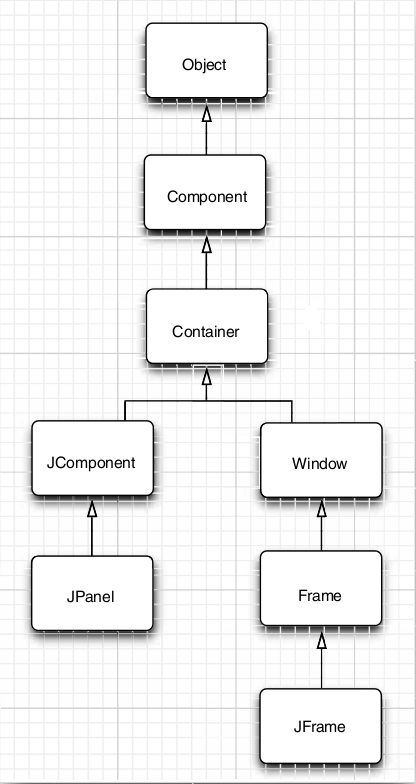
\includegraphics[width=320px,height=160px]{images/components.png}  
\end{frame}

\begin{frame}{Йерархия}
  \transdissolve
  \begin{itemize}
  \item Window и неговите наследници се вземат от операционна система
  \item JComponent и неговите наследници са Swing GUI компоненти -
    текстови полета, бутони
  \item В Window производните контейнери се поставят Swing компоненти
  \item В JPanel се поставят компоненти, които могат да бъдат групирани
  \end{itemize}
\end{frame}


\begin{frame}{Графика - компоненти}
  \transdissolve
  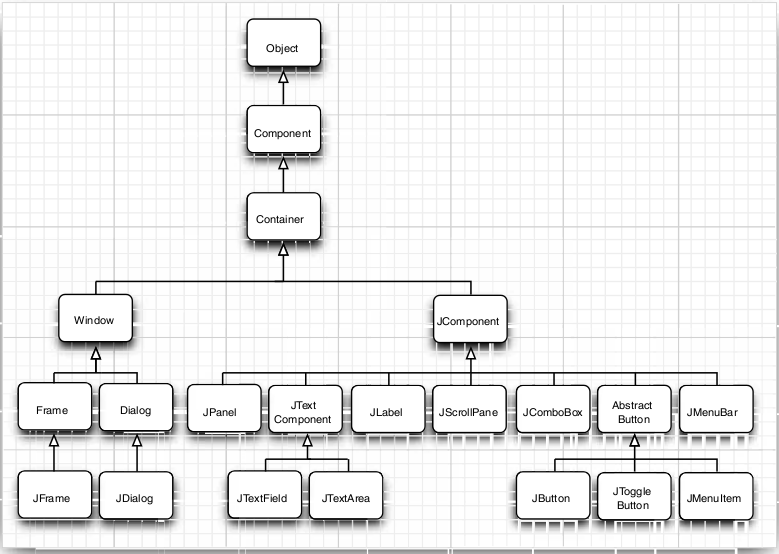
\includegraphics[width=320px,height=160px]{images/all_components.png}
\end{frame}
\section{Позициониране на компоненти}
\subsection{Управление на позиционирането}
\begin{frame}{Позициониране на компоненти в Swing}
  \transdissolve
  \begin{itemize}
  \item Определя позицията на компонентите в даден контейнер
  \item Всеки контейнер има мениджър на позиционирането(layout
    manager) по подразбиране
  \item Препоръчително е той винаги да бъде инстанциран изрично
  \end{itemize}
\end{frame}

\subsection{Flow layout}
\begin{frame}[fragile]
  \frametitle{Пример - flow layout}
  \transdissolve
\begin{lstlisting}
JFrame frame = new JFrame();
frame.setSize(600, 400);
JPanel panel = new JPanel();
panel.setLayout(new FlowLayout());
frame.add(panel);
panel.add(new JButton("Button1"));
\end{lstlisting}
\end{frame}

\subsection{Border layout}
\begin{frame}{Border layout}
  \transdissolve
  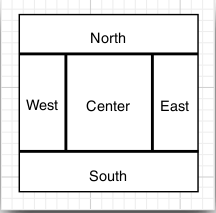
\includegraphics[width=160px,height=160px]{images/border_layout.png}
\end{frame}

\begin{frame}[fragile]
  \frametitle{Пример - border layout}
  \transdissolve
\begin{lstlisting}
JPanel panel = new JPanel();
panel.add(yellowButton);
panel.add(blueButton);
panel.add(redButton);
frame.add(panel, BorderLayout.SOUTH);  
\end{lstlisting}
\end{frame}

\subsection{Grid layout}
\begin{frame}[fragile]
  \frametitle{Пример - grid layout}
  \transdissolve
\begin{lstlisting}
panel.setLayout(new GridLayout(5, 4));
panel.add(new JButton("1"));
panel.add(new JButton("2"));  
\end{lstlisting}
\end{frame}

\section{Основни компоненти}

\begin{frame}{Основни компоненти}
  \transdissolve
  \begin{itemize}
  \item Текстово поле(JTextField)
  \item Многоредов текстов компонент(JTextArea)
  \item Бутон(JButton)
  \item Компонент за множествен избор(JComboBox)
  \end{itemize}
\end{frame}

\section{Обработка на събития}

\begin{frame}{Обработка на събития}
  \transdissolve
  \begin{itemize}
    \item Слушател за събитие(Action Listener)
    \begin{itemize}
    \item Инстанция на клас, който реализира Listener интерфейс.
    \end{itemize}
    \item Източник на събитие(Event Source)
      \begin{itemize}
      \item Обект(компонент), към който могат да бъдат прикачани слушатели, на
        които да бъдат предавани събития        
      \end{itemize}
    \item Събития в Swing
      \begin{itemize}
      \item обикновено възникват в резултат от взаимодействието
        между приложението и потребителят
      \item натискане на бутон, загуба на фокус, минимизиране на прозорец и т.н.
      \end{itemize}
  \end{itemize}
\end{frame}

\begin{frame}{Връзка между източник и слушател}
  \transdissolve
  \begin{itemize}
  \item Източникът генерира събития
  \item Слушателят се регистрира(абонира) за тези събития
  \item Един източник може да има много слушатели
  \item Един слушател може да е регистриран към много източници
  \item Слушателят реагира на базата на полученото съобщение
  \item Шаблон за дизайн Наблюдател(Observer)
  \end{itemize}
\end{frame}


\begin{frame}{Източник слушател - диаграма}
  \transdissolve
  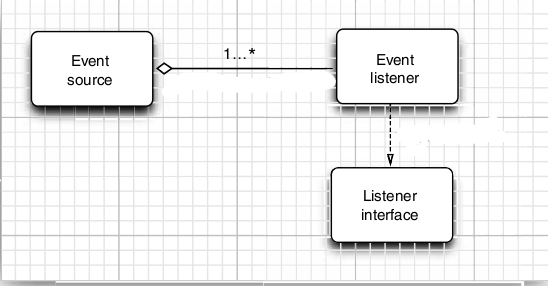
\includegraphics[width=320px,height=160px]{images/event_source.png}  
\end{frame}

\begin{frame}{Обработка на събития - диаграма}
  \transdissolve
  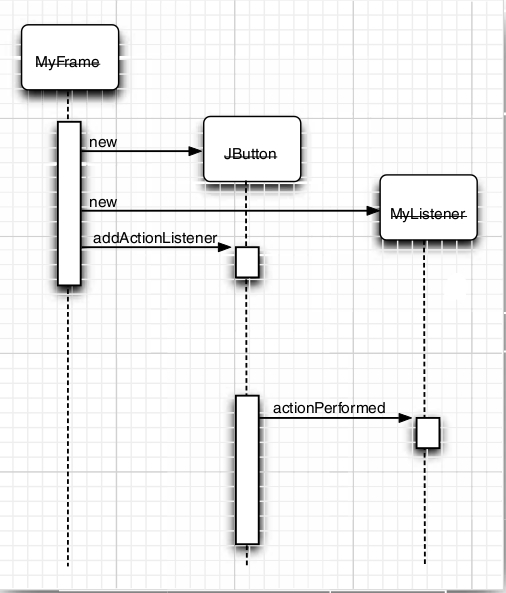
\includegraphics[width=320px,height=160px]{images/event_handling.png}  
\end{frame}

\begin{frame}[fragile]
  \frametitle{Пример}
  \transdissolve
\begin{lstlisting}
frame.addWindowListener(new WindowListener() { // listener
  public void windowOpened(WindowEvent e) {
    System.out.println("Window opened"); 
  }
  
  public void windowClosed(WindowEvent e) {
    System.out.println("Window closed"); 
  }
}

\end{lstlisting}
\end{frame}

\begin{frame}{Адаптерни класове}
  \transdissolve
  \begin{itemize}
  \item Някои Listener интерфейси съдържат много методи
  \item Обикновено повечето от тях не ни интересуват
  \item Интерфейсът задължава да бъдат реализирани всичките му класове
  \item Адаптерните класове предлагат празна имплементация на всички
    интерфейсни методи
  \item Подходящи винаги, когато да реализираме само част от методите
  \end{itemize}
\end{frame}


\begin{frame}{Йерархия на събитията в Swing}
  \transdissolve
  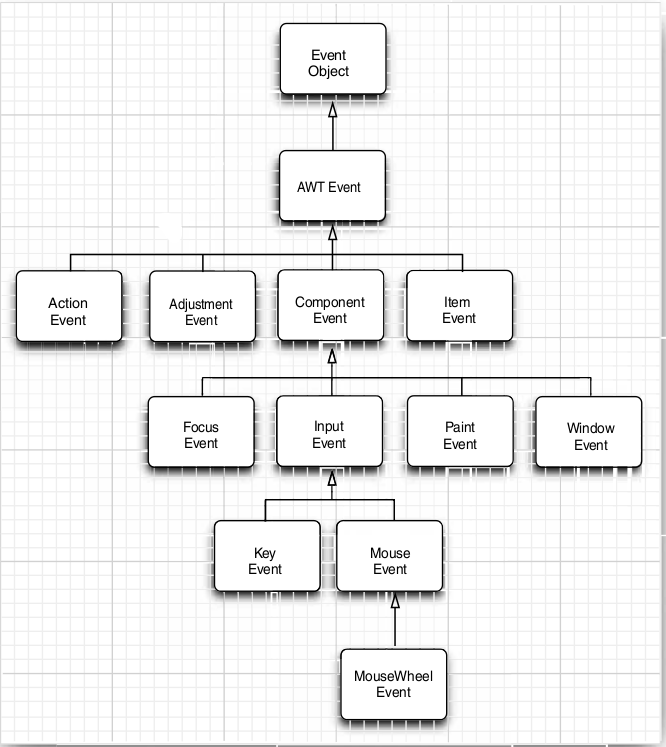
\includegraphics[width=320px,height=160px]{images/events.png}  
\end{frame}

\begin{frame}{Основни събития}
  \transdissolve
  \begin{itemize}
  \item ActionEvent
  \item AdjustmentEvent
  \item ItemEvent
  \item KeyEvent
  \item MouseEvent
  \item MouseWheelEvent
  \item FocusEvent
  \item WindowEvent
  \end{itemize}
\end{frame}

\begin{frame}{Основни Listener интерфейси}
  \transdissolve
  \begin{columns}
    \column{.5\textwidth}
    \begin{itemize}
      \item ActionListener
      \item AdjustmentListener
      \item FocusListener
      \item ItemListener
      \item KeyListener
      \item MouseListener
    \end{itemize}
    \column{.5\textwidth}
    \begin{itemize}
      \item MouseMotionListener
      \item MouseWheelListener
      \item WindowListener
      \item WindowFocusListener
      \item WindowStateListener
    \end{itemize}

  \end{columns}
\end{frame}

\begin{frame}{Адаптерни класове}
  \transdissolve
  \begin{itemize}
  \item FocusAdapter
  \item KeyAdapter
  \item MouseAdapter
  \item MouseMotionAdapter
  \item WindowAdapter
  \end{itemize}
\end{frame}

\section*{Заключение}

\begin{frame}{Заключение}
  \transdissolve
  % Keep the summary *very short*.
  \begin{itemize}
  \item
    Swing е една от най-добрите библиотеки за създаване на портативни
    графични интерфейси.
  \item
    Обработката на съобщения е в сърцето и.
  \item
    За пълноценна работа с езикът и платформата Java човек трябва да
    се запознае с доста инструменти.
  \end{itemize}
  
  % The following outlook is optional.
  \vskip0pt plus.5fill
  \begin{itemize}
  \item
    Следващият път:
    \begin{itemize}
    \item
      Стандартни Swing компоненти
    \item
      MiG layout
    \end{itemize}
  \end{itemize}
\end{frame}

\begin{frame}{Въпроси}
  \transdissolve
  \begin{center}
    \LARGEТук е момента да зададете вашите въпроси! :-)
  \end{center}
\end{frame}

\begin{frame}{Край}
  \transdissolve
  \begin{center}
    \LARGEБлагодаря Ви за вниманието!
  \end{center}
\end{frame}

\end{document}

%%% Local Variables: 
%%% mode: latex
%%% TeX-master: t
%%% End: 
